\section{Appendix}

Figure~\ref{fig:switch_resources} provides a breakdown of the resource
consumption of Swordboxes components. We collected these values from our
experimental setup on an Edge Core Wedge 100BF-65X using the barefoot SDE
version 9.7.0. Each reported percentage is the average value across the total 16
switch pipeline stages. {\sword} fits into 8 stages, and is run entirely on the
ingress pipeline.

\textbf{Switch Resource Utilization}
\begin{figure}[t]
    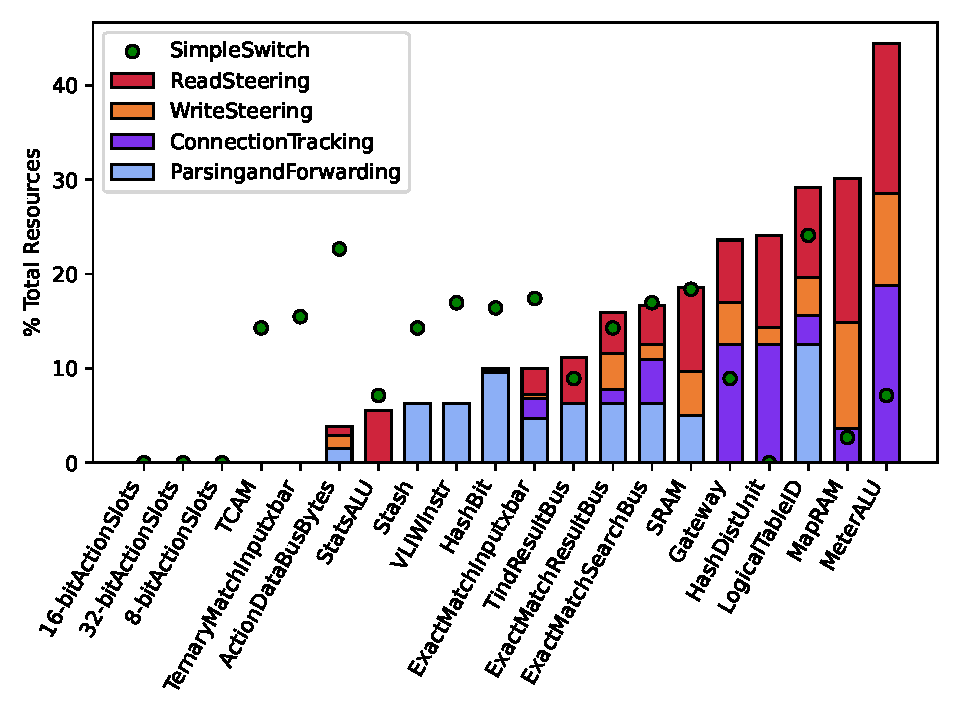
\includegraphics[width=0.485\textwidth]{fig/switch_resources.pdf}
%  \vskip -0.5em
    \caption{Breakdown of switch resource utilization by swordbox component}
    \label{fig:switch_resources}
%      \vskip -0.5em
\end{figure}

\subsection{Packet Size}
\todo{Write about packet sizes}

\begin{figure}
  \centering
  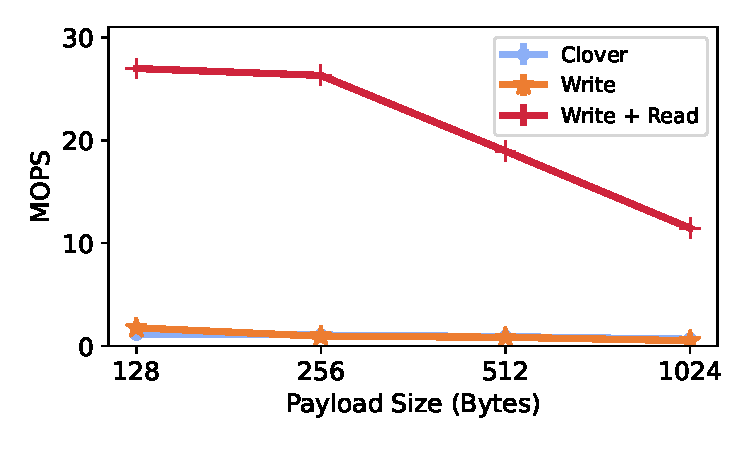
\includegraphics[width=0.485\textwidth]{fig/packet_size.pdf}

    \caption{Performance across RDMA payload sizes using 120 client cores at a 50 percent read 50 percent write ratio.}

    \label{fig:packet_size}
\end{figure}

\subsection{Contention}
\todo{Write about contention}
\begin{figure}
  \centering
  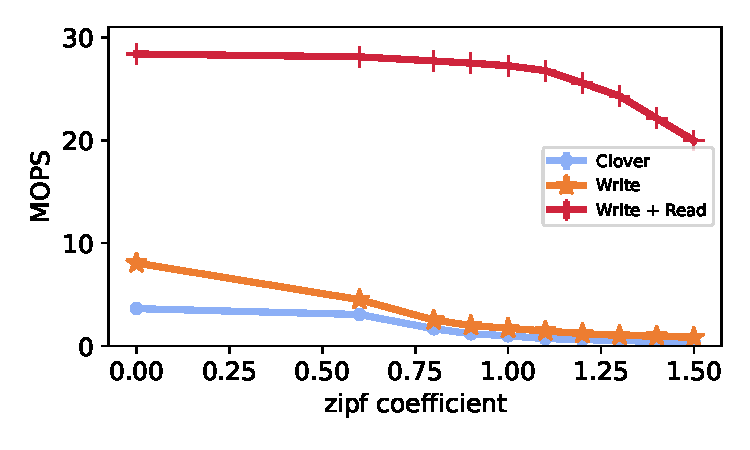
\includegraphics[width=0.485\textwidth]{fig/contention.pdf}

    \caption{Performance as contention increases with zipf coefficient using 120 client cores.
    \todo{These numbers need to be extended to 400 cores}}

    \label{fig:packet_size}
\end{figure}
